\section{}
Consider the steady flow of water through an axisymmetric garden hose nozzle shown below. The axial component of velocity increases linearly from $u_{z,entrance}$ to $u_{z,exit}$ as sketched. Between $z = 0$ and $z = L$, the axial velocity component is given by $u_z = u_{z,entrance} + [(u_{z,exit} - u_{z,entrance})/L]z$. Generate an expression for the radial velocity component $u_r$ between $z = 0$ and $z = L$. You may ignore frictional effects on the walls.
\begin{figure}[h]
    \centering
    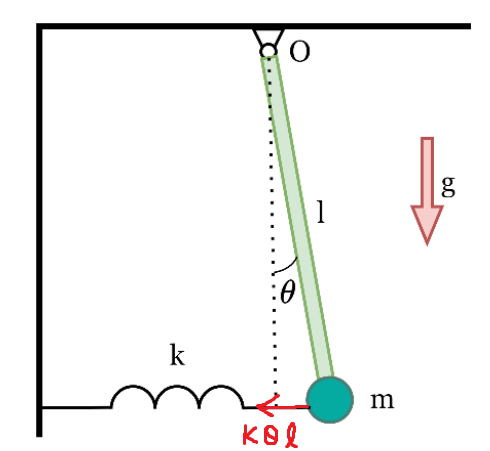
\includegraphics[width=0.5\textwidth]{Questions/Figures/q3 problem diagram.png}
    \caption{Garden hose nozzle}
\end{figure}

\subsection*{Solution}
First we list assumptions
\begin{table}[h]
    \centering
    \caption{Assumptions}
    \begin{tabular}{c|c}
        Assumption & Approximation \\
        \hline
        Steady flow & $\partial_t = 0$ \\
        Incompressible flow & $\rho = \text{constant}$ \\
        Axisymmetric flow & $\partial_{\theta} = 0$ \\
        No friction & $\tau_{w} = 0$ \\
        No heat transfer & $q = 0$ \\
        No body forces & $\mathbf{F} = 0$ \\
    \end{tabular}
\end{table}
\FloatBarrier
The continuity equation for incompressible flow is given by
\begin{align*}
    \nabla \cdot \vec{v} = 0
\end{align*}
In cylindrical coordinates, the continuity equation is given by
\begin{align*}
    \frac{1}{r} \frac{\partial}{\partial r}(r u_r) + \cancelto{\text{axisymmetric}}{\frac{1}{r}\frac{\partial}{\partial \theta}(u_{\theta})} + \frac{\partial}{\partial z}(u_z) &= 0 \\
\end{align*}
Substituting the given expression for $u_z$ into the continuity equation, we have
\begin{align*}
    \frac{1}{r} \frac{\partial}{\partial r}(r u_r) + \frac{\partial}{\partial z}\left(u_{z,entrance} + \frac{u_{z,exit} - u_{z,entrance}}{L}z\right) &= 0 \\
    \frac{1}{r} \frac{\partial}{\partial r}(r u_r) + \frac{u_{z,exit} - u_{z,entrance}}{L} &= 0 
\end{align*}
Solving for $u_r$, we have
\begin{align*}
    \frac{\partial}{\partial r}(r u_r) &= -\left(u_{z,exit} - u_{z,entrance}\right)\frac{r}{L} \\
    r u_r &= -\frac{r^2}{2L}\left(u_{z,exit} + \frac{r^2}{2L}u_{z,entrance}\right) + g(z) 
\end{align*}
Notice that at $r=0$, 
\begin{align*}
    (0)u_r &= -\frac{0^2}{2L}\left(u_{z,exit} + \frac{0^2}{2L}u_{z,entrance}\right) + g(z) \\
    \implies g(z) &= 0
\end{align*}
Thus, the radial velocity component is given by
\begin{align*}
    \Aboxed{u_r &= -\frac{r}{2L}\left(u_{z,exit} + \frac{r^2}{2L}u_{z,entrance}\right)}
\end{align*}
